\documentclass[journal]{IEEEtran}

\usepackage{tabularx}
\usepackage{varioref}
\usepackage{subfigure}
\usepackage{color}

\usepackage{xspace}
\usepackage{amsmath}
\usepackage{capt-of}
\usepackage{caption}
\usepackage{listings}
\usepackage{array}
\usepackage{ragged2e}
\usepackage{booktabs}
\usepackage{float}
\usepackage{colortbl}
\usepackage{algorithm2e}

\newcommand{\PreserveBackslash}[1]{\let\temp=\\#1\let\\=\temp}
\newcolumntype{L}[1]{>{\PreserveBackslash\RaggedRight}p{#1}}
\newcolumntype{R}[1]{>{\PreserveBackslash\RaggedLeft}p{#1}}

\definecolor{orange}{rgb}{1,0.5,0}

\ifx\pdfoutput\undefined
\usepackage{graphicx}
\else
\usepackage[pdftex]{graphicx}
\fi

\hyphenation{op-tical net-works semi-conduc-tor}


\begin{document}
\newcommand{\ra}[1]{\renewcommand{\arraystretch}{#1}}

\title{A Group Mobility Model Generator for MANETs Using Terrain Maps}

\author{Hagen~Paul~Pfeifer\\Furtwangen University\\Faculty of Business
Information Systems\\hagen.pfeifer@hs-furtwangen.de}



\markboth{\today{} --- Munich}{}
\maketitle


\begin{abstract}
A genetic algorithm is chosen to calculate the ideal configuration for every
Condition Class. All kind of calculated intervals and hold-times are guarded
through pre-defined upper and lower thresholds guarantee a complaisant protocol
behavior.
\end{abstract}

% 
\begin{keywords}
Genetic algorithms, Software performance, Functional analysis
\end{keywords}
% 
\IEEEpeerreviewmaketitle


%%%%%%%%%%%%%%%%%%%%%%%%%%%%%%%%%%%%%%%
\section{Introduction}


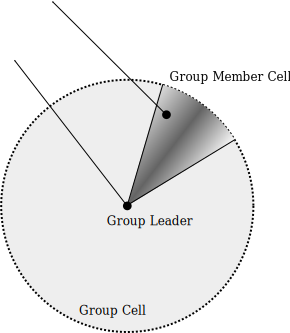
\includegraphics[width=.7\linewidth]{figures/macro-mobility.pdf}

%%%%%%%%%%%%%%%%%%%%%%%%%%%%%%%%%%%%%%%
\section{Functioning}


%%%%%%%%%%%
\subsection{Mode of operation}

\begin{algorithm}[H]
  \SetLine
  parse scenario file\;
	generate random terrain map\;
  \While{each defined group leader}{
		determine group leader route
	}
  \caption{How to write algorithms}
\end{algorithm}

\begin{algorithm}[H]
  \SetLine
  \KwData{this text}
  \KwResult{how to write algorithm with \LaTeX2e }
  initialization\;
  \While{not at end of this document}{
    read current\;
    \eIf{understand}{
      go to next section\;
      current section becomes this one\;
      }{
      go back to the beginning of current section\;
      }
    }
  \caption{How to write algorithms}
\end{algorithm}

%%%%%%%%%%%
\subsection{Terrain Penalty Map}

\begin{figure}
    \centering
    \subfigure[50000m]{\includegraphics[width=0.24\textwidth]{figures/penalty-map-3d.pdf}}
    \subfigure[25000m]{\includegraphics[width=0.24\textwidth]{figures/penalty-map-3d-flat.pdf}}\\
     %
    \caption{Terrain Penalty Map}%
    \label{fig:terrain-penalty-map}
\end{figure}

%%%%%%%%%%%
\subsection{Group Leader}

Gravity Penalty

%%%%%%%%%%%%%%%%%%%%
\section{Conclusion}


\nocite{*}
\bibliography{literature}
\bibliographystyle{plain}


\end{document}
